\documentclass[12pt]{article}
\usepackage[margin=2cm]{geometry} 
\usepackage{titling}
\usepackage{graphicx}
\usepackage{float}
\usepackage[hidelinks]{hyperref}
\usepackage[italian]{babel}
\usepackage{subcaption}

\setlength\parindent{0pt}
\setlength{\parskip}{1em}
\setlength{\droptitle}{-2cm}

\title{Istruzioni d'uso AR Sandbox (ad uso interno)}
\author{Università della Svizzera italiana}
\date{Versione \today}


\begin{document}
\maketitle
\tableofcontents
\newpage


\section{Installazione}\label{installation}	

	\subsection{Componenti}
	
		\begin{itemize}
			\item PC
			\item Cavo DVI lungo e 2x cavo alimentazione
			\item Proiettore
			\item Kinect v2
			\item Materiale di montaggio Kinect e proiettore
			\item (opzionale) Altoparlanti
		\end{itemize}
		
		
	\subsection{Montaggio}
	
		\begin{enumerate}
			\item Collegare l'alimentazione e il cavo DVI al proiettore (entrata MONO 2D)
			\item Montare il proiettore sull'apposito supporto e far passare i cavi
			nell'apertura
			\item Montare il Kinect sul supporto dedicato e far passare il cavo nell'apertura
			\item Collegare l'alimentazione e il cavo DVI al PC, ed eventualmente gli altoparlanti
			\item Collegare l'alimentazione del Kinect e il cavo USB (blu) ad una porta USB 3.0 (blu) del PC
		\end{enumerate}

		\begin{figure}[H]
			\centering
			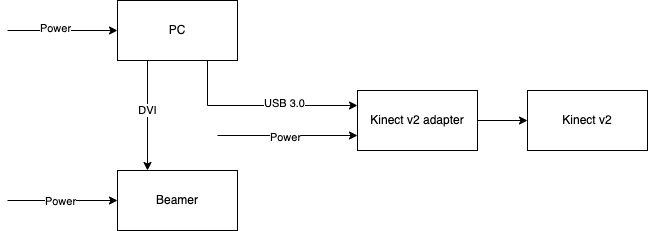
\includegraphics[width=0.9\textwidth]{img/cablesScheme.png}
			\caption*{Lo schema dei cavi}
		\end{figure}

		\begin{figure}[H]
			\centering
			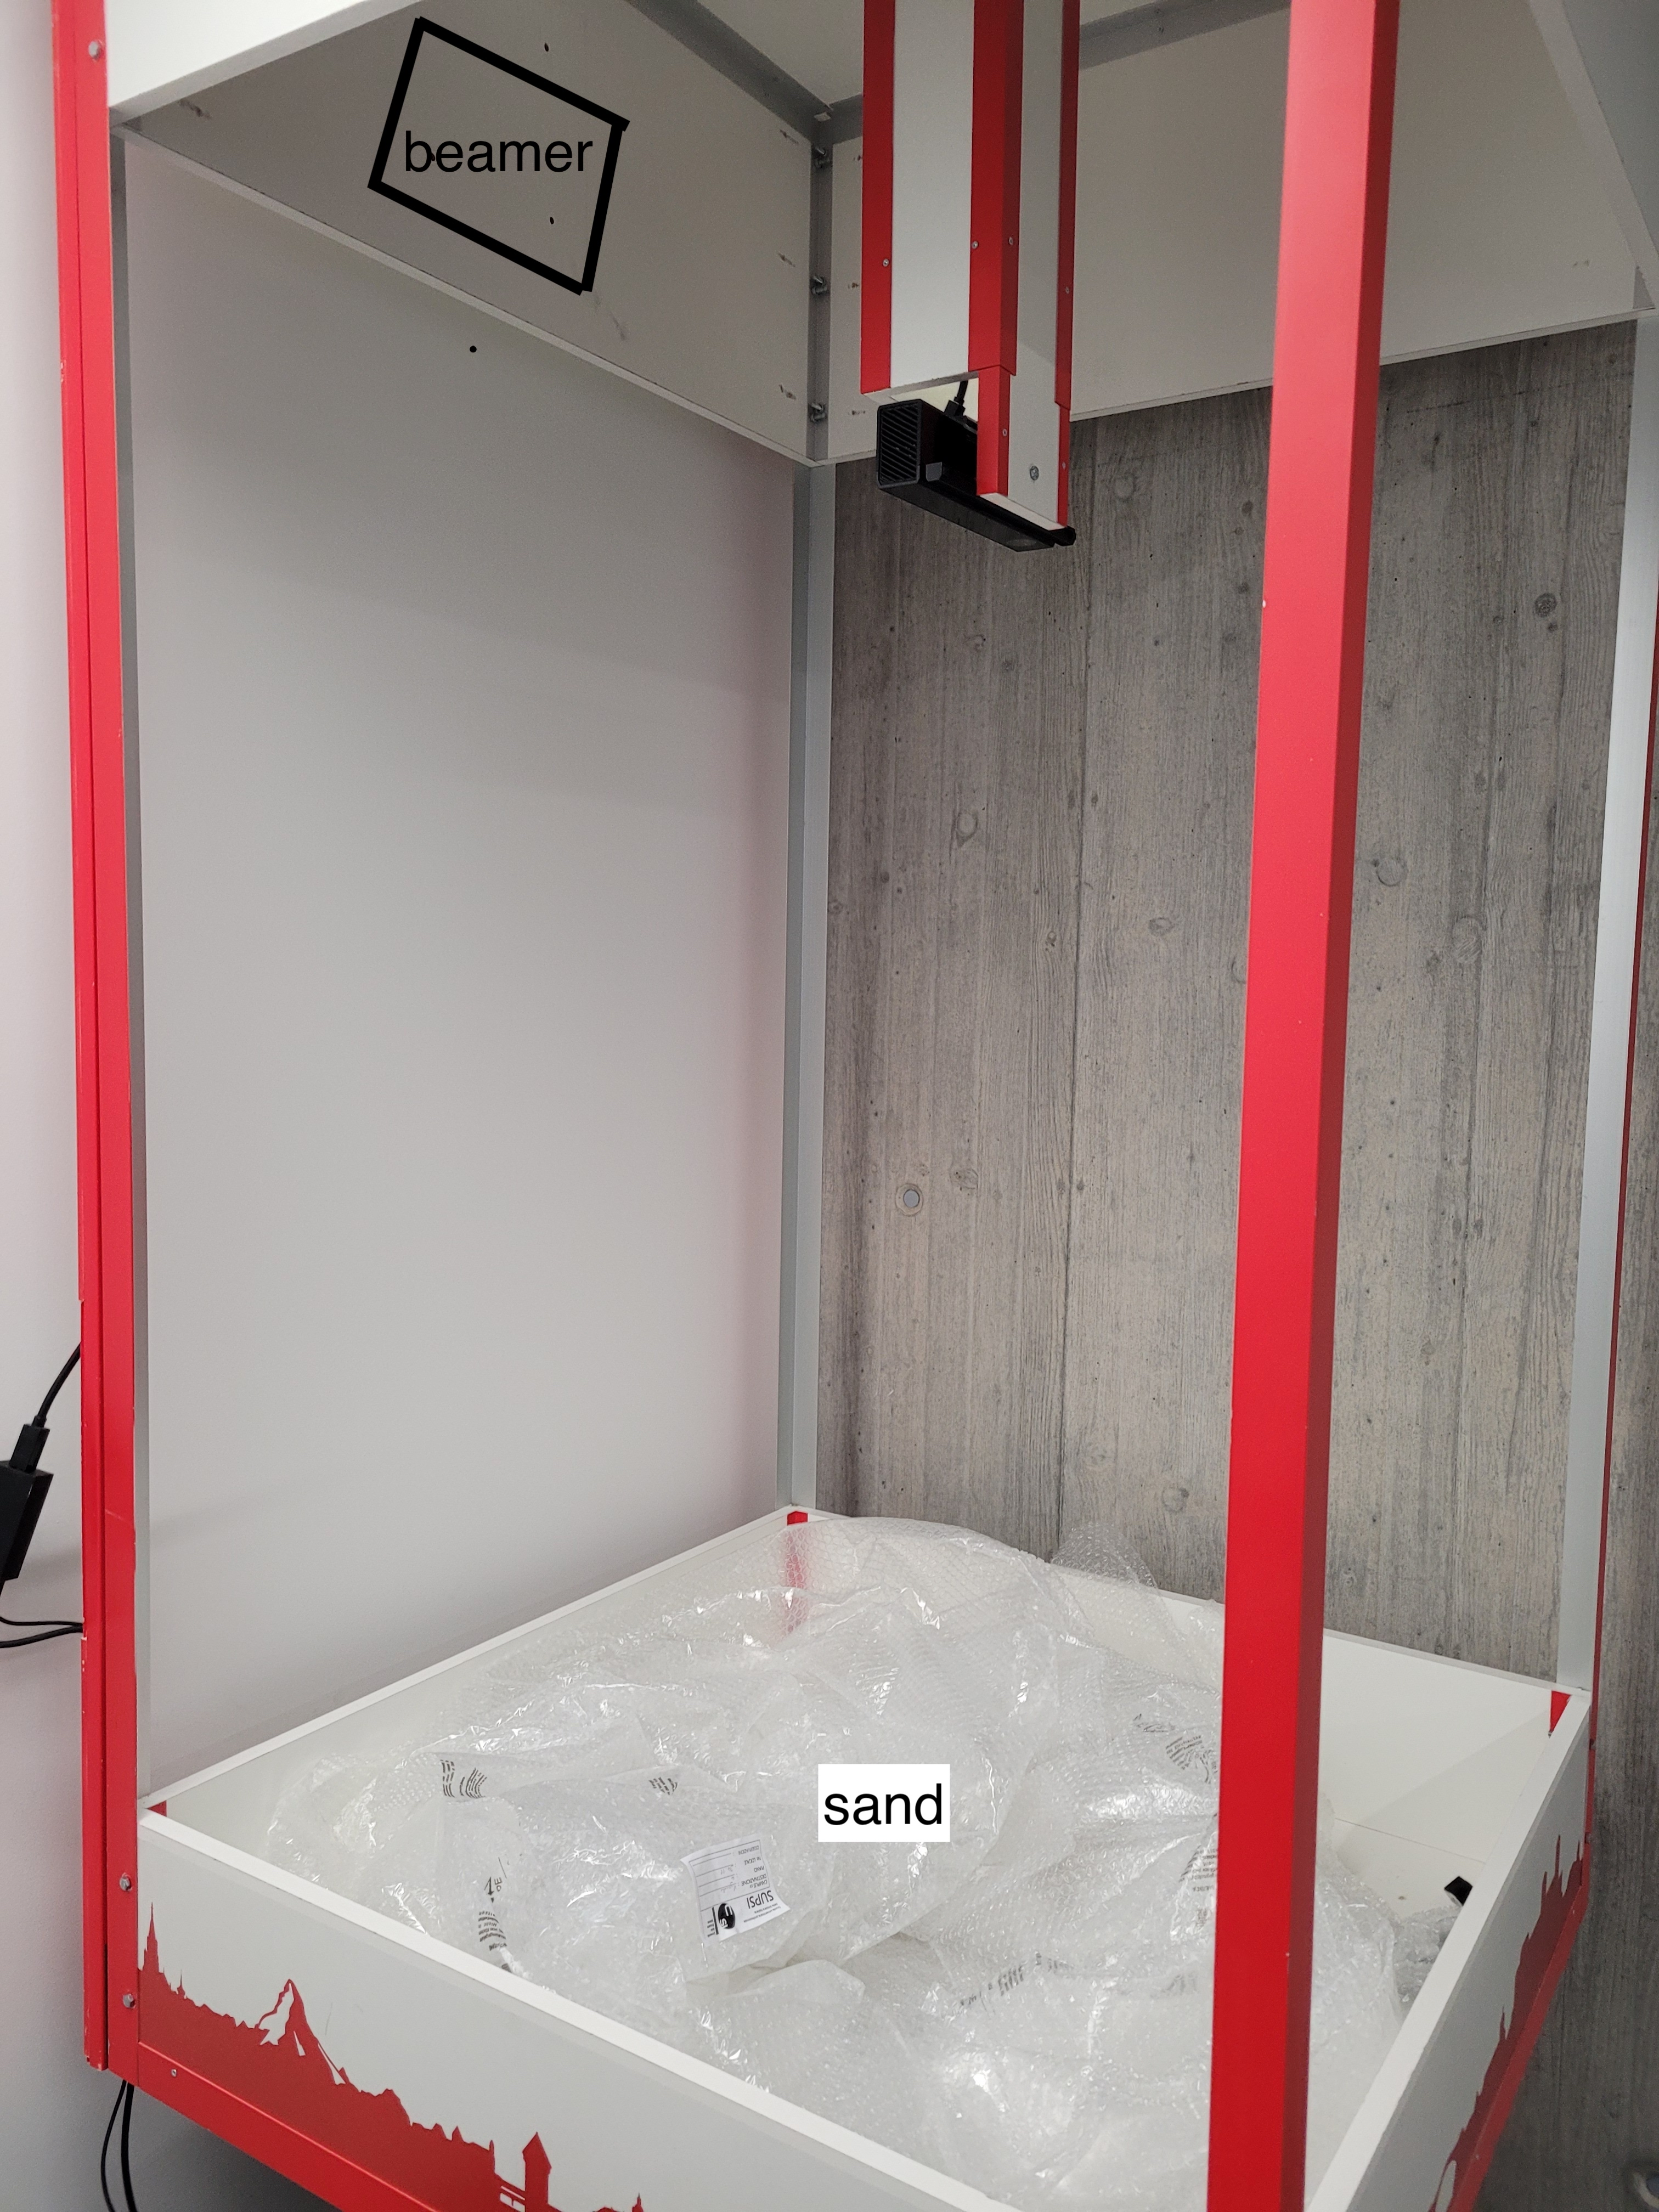
\includegraphics[width=0.9\textwidth]{img/sandbox.jpg}
			\caption*{La sandbox assemblata}
		\end{figure}
		
		
	\subsection{Avvio}

		Accendere il proiettore, dopodiché avviare il PC e cliccare sul collegamento
		\texttt{ARSandBox} sul Desktop. Controllare che il proiettore \textbf{non} sia in modalità 3D
		(menu $\rightarrow$ stereo $\rightarrow$ stereo mode).\\

		Se l'immagine dovesse essere calibrata correttamente (con spazio è possibile vedere 
		un'anteprima), premere F5 per uscire dalla modalità setup.

	\subsection{Spegnimento}
		
		Premere ESC per uscire dal programma, dopodiché arrestare normalmente il sistema e 
		premere due volte il tasto \texttt{Power} del beamer per spegnerlo. \textbf{NON} scollegarlo finché
		il LED arancione lampeggia (raffreddamento in corso)!
		
		
\section{Utilizzo}

	\subsection{Tasti utili}
	
	\begin{tabular}{l l}
		ESC & esci\\
		P & salva mesh\\
		F5 & chiudi modalità setup\\
		- & mostra solo terreno\\
	\end{tabular}

	In modalità setup

	\begin{tabular}{l l}
		Shift & movimento più lento\\

		F1 & terreno 1\\
		F2 & terreno 2\\
		F3 & terreno 3\\

		1/2/3/4 & seleziona angoli\\
		5 & ridimensiona terreno\\
		6 & muovi terreno\\

		W/A/S/D & sposta il terreno nella direzione corrispondente\\

		Space & entra in modalità calibrazione Kinect/proiettore\\

		9 & salva calibrazione su disco\\
		0 & carica calibrazione dal disco\\

		U/J & aumenta/riduci l'altezza minima\\
		I/K & aumenta/riduci l'altezza massima\\
	\end{tabular}
		
		
\section{Codice sorgente}

	Il codice sorgente dell'applicazione, assieme alle istruzioni per compilarla, si trova alla pagina \url{https://github.com/USI-Showroom/ARSandbox}.
		
	
\end{document}
